\chapter{Resultados}
\label{chap:result}

O desenvolvimento do portfólio digital resultou em um produto funcional e alinhado às expectativas do cliente. A seguir, são apresentados os principais resultados alcançados durante o projeto.

% %--------- NEW SECTION ----------------------
% \section{Testes unitários}
% \label{sec:testu}
% \lipsum[1]

% \section{Integração do sistema}
% \label{sec:intsis}
% \lipsum[1]

% %--------- NEW SECTION ----------------------
% \section{Testes integrados}
% \label{sec:testi}
% \lipsum[1]

\section{Diagrama de classes}
\label{sec:class}
O diagrama de classes é uma representação visual das classes do sistema e seus relacionamentos. Ele é utilizado para descrever a estrutura do sistema e como as classes interagem entre si. A Figura \ref{fig:diagrama-classes} apresenta o diagrama de classes do sistema desenvolvido.

\begin{figure}[H]
    \centering
    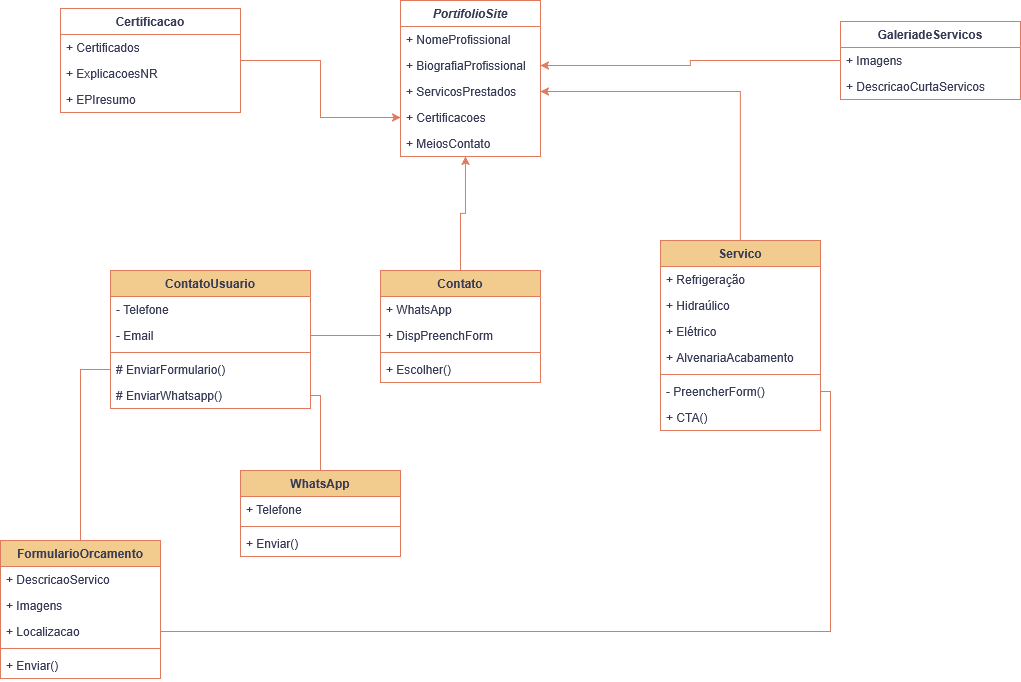
\includegraphics[width=0.6\textwidth]{Figures/Diagrama_de_classes.png} % use your image path and name here
    \caption{Diagrama de classes.}
    \label{fig:diagrama-classes}
\end{figure}

\section{Diagrama de casos de uso}
\label{sec:casos}
O diagrama de casos de uso é uma representação visual das funcionalidades do sistema e como os usuários interagem com ele. Ele é utilizado para descrever os requisitos funcionais do sistema e identificar os atores envolvidos. A Figura \ref{fig:diagrama-uso} apresenta o diagrama de casos de uso do sistema desenvolvido.

\begin{figure}[H]
    \centering
    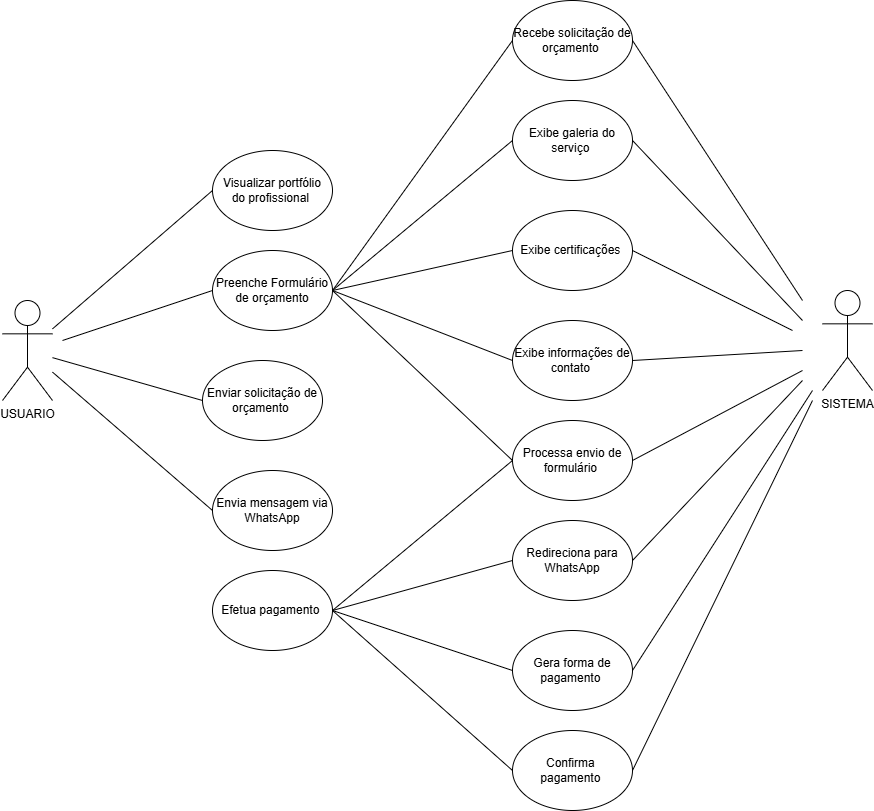
\includegraphics[width=0.6\textwidth]{Figures/Diagrama_de_uso.png} % use your image path and name here
    \caption{Diagrama de casos de uso.}
    \label{fig:diagrama-uso}
\end{figure}


\section{Diagrama de sequência}
\label{sec:sequencia}   
O diagrama de sequência é uma representação visual das interações entre os objetos do sistema ao longo do tempo. Ele é utilizado para descrever o fluxo de mensagens entre os objetos e como eles colaboram para realizar uma funcionalidade específica. A Figura \ref{fig:diagrama-sequencia} apresenta o diagrama de sequência do sistema desenvolvido.

\begin{figure}[H]
    \centering
    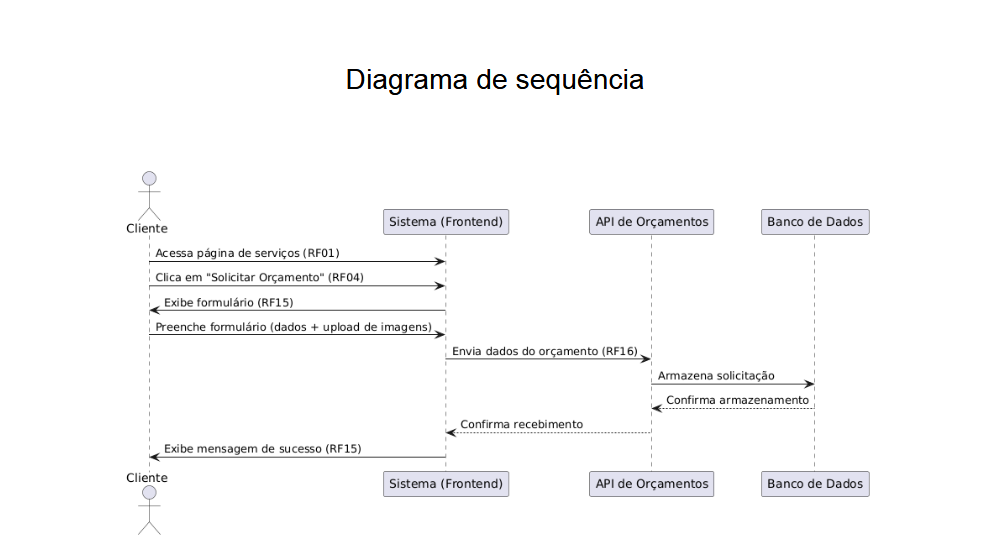
\includegraphics[width=0.6\textwidth]{Figures/seq.png} % use your image path and name here
    \caption{Diagrama de sequência.}
    \label{fig:diagrama-sequencia}
\end{figure}

O cliente inicia o processo acessando a página onde os serviços são destacados e, em seguida, clica no botão "Solicitar Orçamento". Ao realizar essa ação, é apresentado um formulário inteligente, no qual o sistema exibe campos para que o cliente possa inserir a descrição do serviço, fazer o upload de imagens e informar a localização. Após o cliente preencher e enviar esses dados, ocorre a integração com uma API: o sistema envia as informações para a API de orçamentos, que pode ser tanto do WhatsApp quanto uma API independente. Essa API, por sua vez, armazena os dados recebidos no banco de dados e retorna uma confirmação. Como feedback, o sistema exibe uma mensagem de sucesso para o cliente, finalizando a solicitação.










